\chapter{Energy Estimation} 
\label{chapter-energy-estimation} 

In the introduction we suggested that a mode of the input sample that is significantly different from the training distribution may cause undesired activations in the neural network, i.e. the failure intensity of a mode is correlated with its likelihood relative to the training distribution. Furthermore, in Section \ref{sec:ebm} we explained that the energy function in energy-based models is proportional to the negative log-likelihood (NLL), which could thus be used to evaluate the failure intensity of a mode. This chapter discusses how to derive the energy function of a denoising autoencoder, which will be used as a metric for the failure intensity (discussed in Chapter \ref{chapter-introduction}).

%----------------------------------------------------------------------------------------
%	SECTION 
%----------------------------------------------------------------------------------------

\section{Autoencoders}

Autoencoders (AE) are models trained to reproduce their inputs to their outputs. An autoencoder is composed of two main parts, the encoder $f$ and the decoder $g$. The input $\mathbf{x} \in  \mathbb{R}^L$ is passed through the encoder $f: \mathbb{R}^L \mapsto \mathbb{R}^U$ as $f(\mathbf{x}) = h(W_f\mathbf{x} + \mathbf{b}_f) = \mathbf{u}$, where $h(\cdot)$ is an activation function applied element-wise and $ \mathbf{u}$ represents the hidden layer. The decoder $g: \mathbb{R}^U \mapsto \mathbb{R}^L$ is then in charge of reconstructing the input, $g(\mathbf{u}) = W_g\mathbf{u} + \mathbf{b}_g$. The output is often called the reconstruction and is written  $r(\mathbf{x}) = g(f(\mathbf{x}))$ with $r: \mathbb{R}^L \mapsto \mathbb{R}^L$. Autoencoders are trained in an unsupervised manner, most of the time using the mean-squared error between input and output as a loss function, $\mathcal{L}_{\text{MSE}} = \lVert r(\mathbf{x}) - \mathbf{x} \rVert_2^2$. Training a model to copy its input may seem useless. To answer this point, we need to distinguish two families of autoencoders, namely undercomplete and overcomplete autoencoders.

\begin{figure}[!h]
\centering
\begin{subfigure}{.5\textwidth}
\vspace*{12mm}
  \centering
  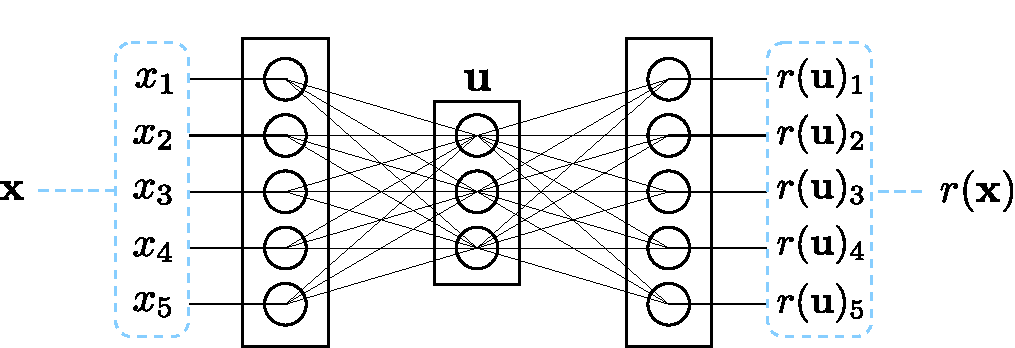
\includegraphics[width=.95\linewidth]{figures/autoencoder-undercomplete}
  \vspace*{8mm}
  \caption{Undercomplete AE}
  \label{fig:undercomplete-ae}
\end{subfigure}%
\begin{subfigure}{.5\textwidth}
  \centering
  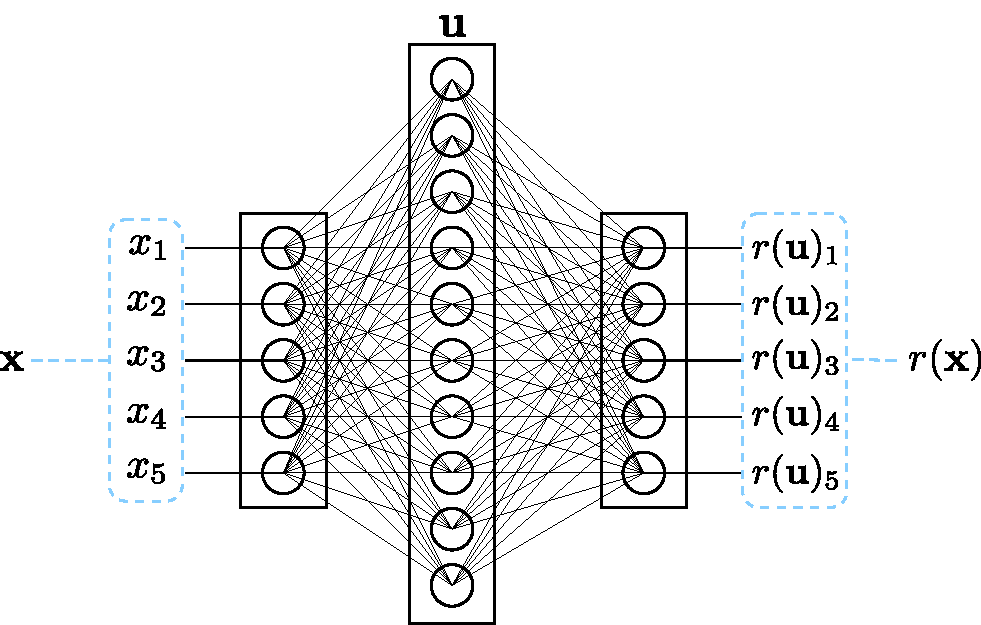
\includegraphics[width=.95\linewidth]{figures/autoencoder-overcomplete}
  \caption{Overcomplete AE}
  \label{fig:overcomplete-ae}
\end{subfigure}
\caption{The architecture of the two families of autoencoders}
\label{fig:under-over-ae}
\end{figure}

%-----------------------------------
%	SUBSECTION 
%-----------------------------------
\subsection*{Undercomplete autoencoders}
An autoencoder is said to be undercomplete when the size of the hidden layer $\mathbf{u}$ is smaller than the size of the input/output layers, i.e. $U < L$ (see Figure \ref{fig:undercomplete-ae}). This amounts to constructing a low-dimensional representation of the input, and information is therefore lost in the process. It can be thought of as a non-linear principal component analysis \citep{pca-ae-1, pca-ae-2} as the values formed in the hidden layer are a non-linear representation in latent space of the input. As can be seen in Figure \ref{fig:reconstruction}, minimizing the mean squared error is similar to minimizing the Euclidean norm of the vector $r(\mathbf{x}) - \mathbf{x}$.
\begin{figure}[!h]
\centering
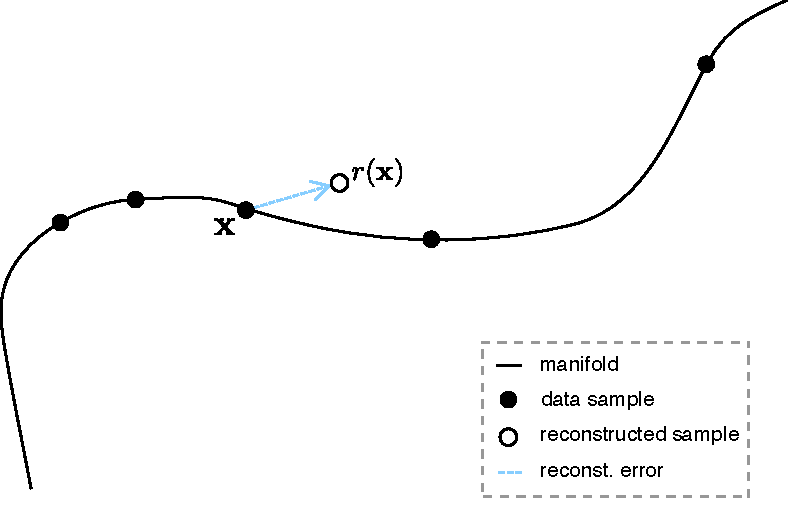
\includegraphics[scale=0.55]{figures/reconstruction}
\caption[Vectorial representation of undercomplete AE]{Vectorial representation of an undercomplete reconstruction process.}
\label{fig:reconstruction}
\end{figure}

%-----------------------------------
%	SUBSECTION 
%-----------------------------------
\subsection*{Overcomplete autoencoders}\label{sec:overcomplete}
Conversely, an overcomplete AE has more hidden units than its input/output layer, i.e. $U > L$ (see Figure \ref{fig:overcomplete-ae}). Hence, the model could thus learn to perfectly copy its input through the $U$ hidden units and reproduce it at the output. However, the input is corrupted before being passed through the encoder, whereas the decoder is forced to reconstruct the original input, i.e. the model learns to denoise signals. This type of AE is called a denoising autoencoder (DAE). More formally, the input is corrupted with some small isotropic noise $\tilde{\mathbf{x}} = \mathbf{x} + \mathbf{\epsilon}$ where $\epsilon \sim \mathcal{N}(0,\,\sigma^{2})$, with the training loss 
\begin{equation}
\mathcal{L}_{\text{MSE}} = \lVert r(\tilde{\mathbf{x}}) - \mathbf{x} \rVert_2^2
\end{equation}
It is worth noticing the difference with the loss function of the undercomplete AE. We verify in Figure \ref{fig:reconstruction-dae} that minimizing the loss implies that the \textit{reconstruction error} $r(\tilde{\mathbf{x}}) - \tilde{\mathbf{x}}$ will converge to $-(\tilde{\mathbf{x}} - \mathbf{x})$ i.e. the model learns to invert the corruption process.

\begin{figure}[!h]
\centering
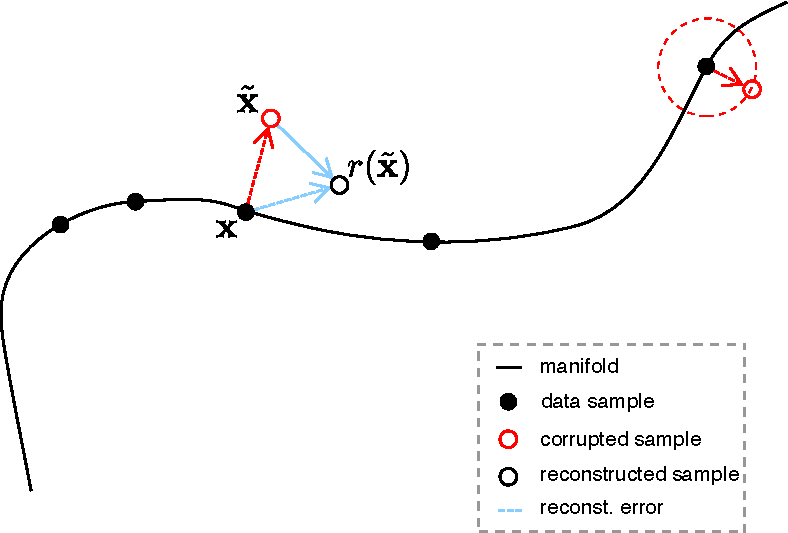
\includegraphics[scale=0.55]{figures/reconstruction-denoising}
\caption[Vectorial representation of overcomplete AE]{Vectorial representation of an overcomplete reconstruction process.}
\label{fig:reconstruction-dae}
\end{figure}

%----------------------------------------------------------------------------------------
%	SECTION 
%----------------------------------------------------------------------------------------

\section{Energy in Autoencoders}

The authors in \citep{alainbengio} found that the reconstruction error of a trained denoising autoencoder is proportional to the score (gradient of log-likelihood)
\begin{equation}
r(\tilde{\mathbf{x}}) - \tilde{\mathbf{x}} \propto \frac{\partial \log p(\tilde{\mathbf{x}})}{\partial \tilde{\mathbf{x}}} 
\label{eq:score-reconstruction}
\end{equation} 
To put it differently, the reconstruction error points towards the corresponding most likely datapoint. This result is not particularly suprising, as denoising a signal is essentially equivalent to finding the most likely datapoint among nearby samples in the distribution (see Figure \ref{fig:reconstruction-dae}). To illustrate Equation (\ref{eq:score-reconstruction}), we train a DAE on a generated circle manifold (more details about this experiment in Section \ref{sec:experiment-I}). As we can see below, the vector field of the reconstruction error does indeed point towards the data manifold\footnote{We refer broadly to a data manifold as a connected set of points that can be approximated well by considering only a small numbers of degrees of freedom.}.
\begin{figure}[!h]
\centering
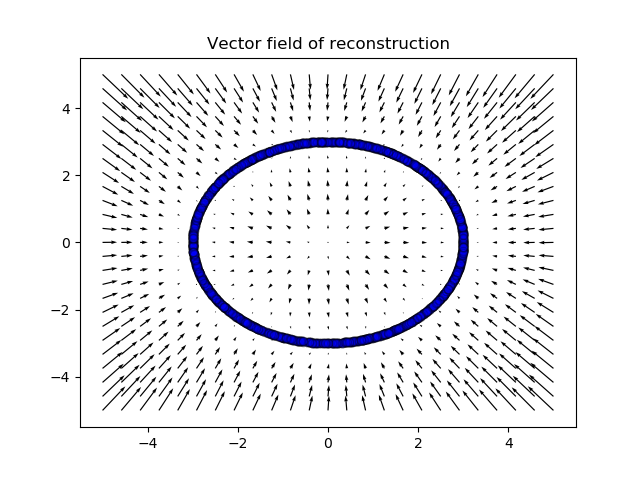
\includegraphics[scale=0.6]{figures/circle-vector-field}
\caption[Vector field circle manifold]{Vector field of reconstruction error on circle manifold. No corruption is applied at test time, the reconstruction error vector is simply the output minus the input. The experimental setup is described in Section \ref{sec:experiment-I}.}
\label{fig:vf-circle}
\end{figure}
Alternatively, Figure \ref{fig:vf-circle} may be interpreted in terms of forces deriving from potential fields as observed in physics. This interpretation can be useful to distinguish the manifold since it acts as a sink in the vector field i.e., has a low potential energy. 

A vector field is the gradient of a potential energy field if it satisfies a simple condition called the integrability criterion\footnote{See Appendix \ref{sec:criterion}}. In \citep{potentialenergy}, the authors found that using tied weights ($W_f = W_g^T = W$), produces an autoencoder configuration whose reconstruction error field satisfies the aforementioned integrability criterion. Indeed, one successively finds
\begin{equation}
\begin{split}
\frac{\partial(r(\tilde{\mathbf{x}})_i- \tilde{x}_i)}{\partial  \tilde{x}_j} &= \frac{\partial\big[W^T h(W\tilde{\mathbf{x}} + \mathbf{b}_f) + \mathbf{b}_g\big]_i}{\partial  \tilde{x}_j} - \frac{\partial\tilde{x}_i}{\partial  \tilde{x}_j} \\
&= \sum_k W_{ik} \frac{\partial h(W\tilde{\mathbf{x}} + \mathbf{b}_f)}{\partial(W\tilde{\mathbf{x}} + \mathbf{b}_f)}W_{jk} - \delta_{ij}   \\
&= \frac{\partial(r(\tilde{\mathbf{x}})_j- \tilde{x}_j)}{\partial  \tilde{x}_i}
\end{split}
\end{equation} 
where $\delta_{ij}$ denotes the Kronecker delta. Hence, under this assumption, the reconstruction error can be expressed as the gradient of a scalar field, the potential energy $-\Psi$, such that $r(\tilde{\mathbf{x}}) - \tilde{\mathbf{x}} = -\partial \Psi(\tilde{\mathbf{x}})/\partial \tilde{\mathbf{x}}$. Thereupon, the reconstruction process can be seen as a gradient descent in the potential energy space \citep{potentialenergy}. A key insight to gain from these developments and Equation (\ref{eq:score-reconstruction}) is that the aforementioned potential energy is in fact proportional to the NLL,
\begin{equation}
\frac{\partial \Psi(\tilde{\mathbf{x}})}{\partial \tilde{\mathbf{x}}} \propto -\frac{\partial \log p(\tilde{\mathbf{x}})}{\partial \tilde{\mathbf{x}}} \Rightarrow  \Psi \propto -\log p
\end{equation}
Since the gradient of the potential energy can be expressed in terms of the reconstruction error, the potential energy $\Psi$ can be computed by integrating the latter,
\begin{equation}
 \Psi(\tilde{\mathbf{x}}) = -\int (r(\tilde{\mathbf{x}}) - \tilde{\mathbf{x}})d\tilde{\mathbf{x}} 
 \label{eq:psi-int}
\end{equation}
Now, expressing $r$ in terms of $f = h(W\mathbf{x} + \mathbf{b}_f)$ and $g = W^Tf(\mathbf{x}) + \mathbf{b}_g$ in (\ref{eq:psi-int}), and following the developments made in \citep{potentialenergy}, we obtain
\begin{equation}
\Psi(\tilde{\mathbf{x}})= -\int f(\tilde{\mathbf{x}})d\tilde{\mathbf{x}} + \frac{1}{2} \lVert \tilde{\mathbf{x}} + \textbf{b}_g \rVert_2^2 + \text{const}
\end{equation} 
In this work only the sigmoid will be used as an activation function $h$, so that the expression of $f$ can be written explicitly and
\newcommand\boxedB[1]{{\setlength\fboxsep{8pt}\boxed{#1}}}
\begin{equation}
\boxedB{\Psi(\tilde{\mathbf{x}}) =  -\sum_k \log(1 + \text{exp}(W_{.k}^T \tilde{\mathbf{x}} + b_k^f)) + \frac{1}{2} \lVert \tilde{\mathbf{x}} - \textbf{b}_g \rVert_2^2 + \cancel{\text{const}} \propto -\log p(\tilde{\mathbf{x}})}
\label{eq:potential-prop}
\end{equation}
where $W_{.k}^T$ is the $k^{\text{th}}$ column of $W^T$, and $b_k^f$ the $k^{\text{th}}$ entry of $\textbf{b}_f$. All intermediate steps between (\ref{eq:psi-int}) and (\ref{eq:potential-prop}) are detailed in \citep{potentialenergy}. It is worth remarking that the potential energy can be negative by construction. 

%----------------------------------------------------------------------------------------
%	SECTION 
%----------------------------------------------------------------------------------------

\section{Experiment I}\label{sec:experiment-I}
In this experiment, two simple data manifolds are generated, on which separate denoising autoencoders are trained. In order to evaluate the suitability of the potential energy as a proxy for the NLL, the former is plotted on a grid for each of these autoencoders.. As a comparison, we also compute the reconstruction error, $\lVert r(\tilde{\mathbf{x}}) - \tilde{\mathbf{x}} \rVert_2^2$, which is sometimes used in the Machine Learning community as a way to detect outliers. 
\subsection*{Manifolds}
The manifolds maps a set of N scalar values $\{t_1, \ldots, t_N\}$ drawn uniformly at random in $[0, 2\pi]$ into a set of vectors $\{\mathbf{x}^1, \ldots, \mathbf{x}^N\} \subset \mathbb{R}^2$. The entries of these vectors are obtained as
$$
\text{wave}  \begin{cases}
      x_1^k = t_k - \pi \\
      x_2^k = \sin(t_k)
    \end{cases}  \qquad \text{circle}  \begin{cases}
     x_1^k = 3\sin(t_k) \\
      x_2^k = 3\cos(t_k)
    \end{cases}
$$
The resulting structures are illustrated in Figure \ref{fig:generate-manifold}.
\begin{figure}[!h]
\centering
\begin{subfigure}{.5\textwidth}
  \centering
  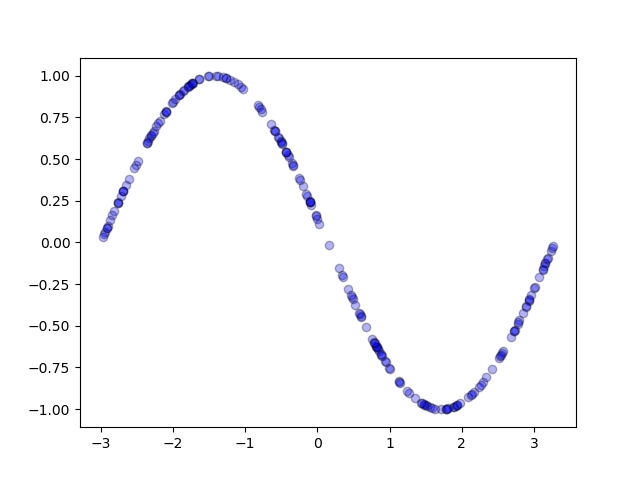
\includegraphics[width=.95\linewidth]{figures/wave-manifold}
  \caption{Wave}
\end{subfigure}%
\begin{subfigure}{.5\textwidth}
  \centering
  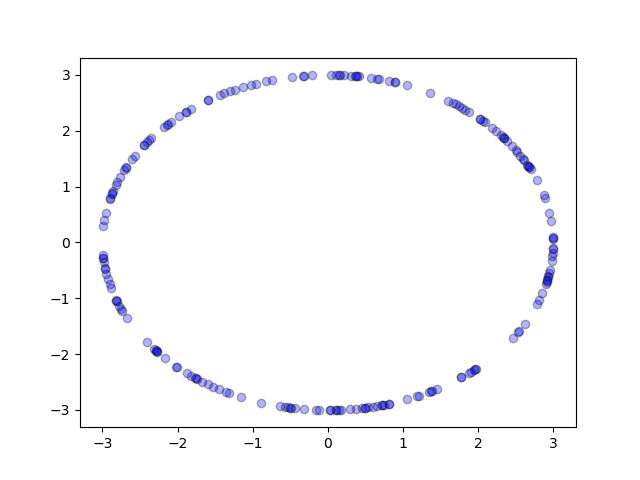
\includegraphics[width=.95\linewidth]{figures/circle-manifold}
  \caption{Circle}
\end{subfigure}
\caption{Manifold generation with 200 samples.}
\label{fig:generate-manifold}
\end{figure}

\subsection*{Setup}
Each autoencoder has 8 hidden units, is trained for 25 epochs, with a batch size of 100, a corruption noise $\sigma = 0.008$ and a learning rate of $1e^{-3}$. The optimizer used is \textit{Adam} \citep{kingma}.

\subsection*{Results}
As expected the vector fields of the reconstruction errors are directed towards the manifolds (see Figure \ref{fig:exp1-vector-fields}), the manifolds acting as sinks. Notably, observe the presence of a source at the origin for the circle manifold (see Figure \ref{fig:exp1-vf-circle}).
\begin{figure}[!h]
\centering
\begin{subfigure}{.5\textwidth}
  \centering
  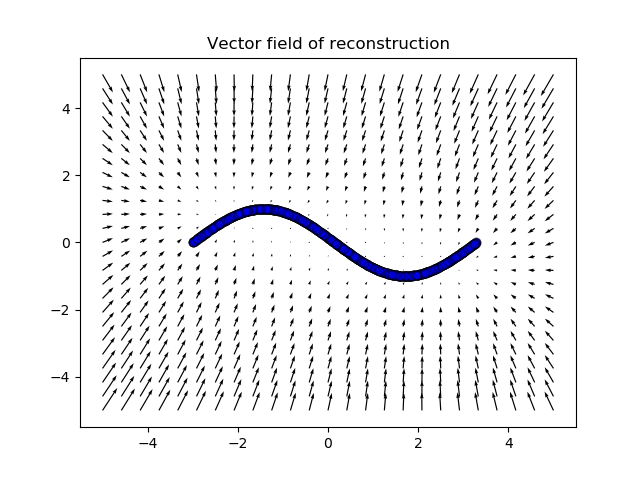
\includegraphics[width=.95\linewidth]{figures/wave-vector-field}
  \caption{Wave}
\end{subfigure}%
\begin{subfigure}{.5\textwidth}
  \centering
  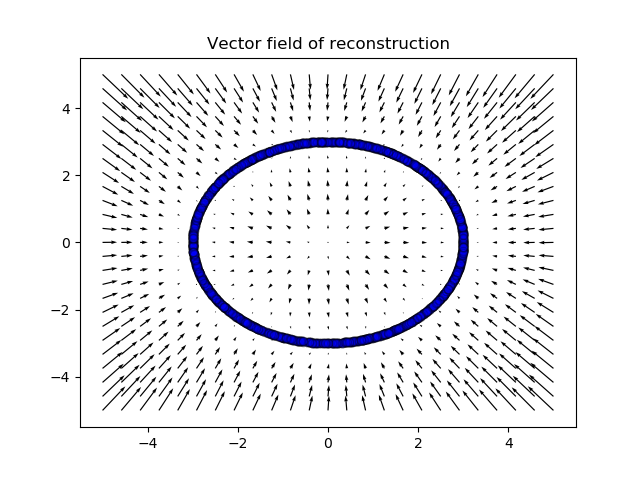
\includegraphics[width=.95\linewidth]{figures/circle-vector-field}
  \caption{Circle}
  \label{fig:exp1-vf-circle}
\end{subfigure}
\caption[Vector fields on wave and circle manifold]{Vector fields of the reconstruction error evaluated on a mesh grid.}
\label{fig:exp1-vector-fields}
\end{figure}

The energy function and the norm of the reconstruction error are computed and plotted onto heatmaps (see Figure \ref{fig:exp1-heatmaps}). We can see that the two estimators have low values in the neighbourhood of the manifold and are high everywhere else. However, the norm of the reconstruction error has also low values at the origin, due to the source in its vector field. This issue makes it difficult in general to use it as a robust criterion to detect and quantify out-of-distribution samples.
\begin{figure}[!h]
\centering
\begin{subfigure}{.5\textwidth}
  \centering
  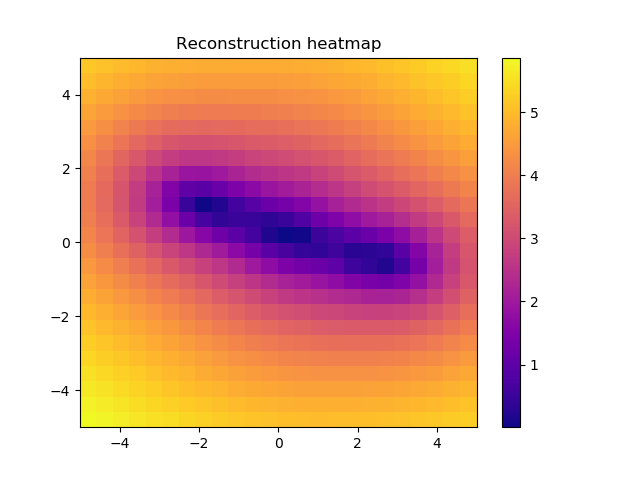
\includegraphics[width=.95\linewidth]{figures/wave-quantifier-reconstruction}
  \caption{Wave - Norm reconstruction error}
\end{subfigure}%
\begin{subfigure}{.5\textwidth}
  \centering
  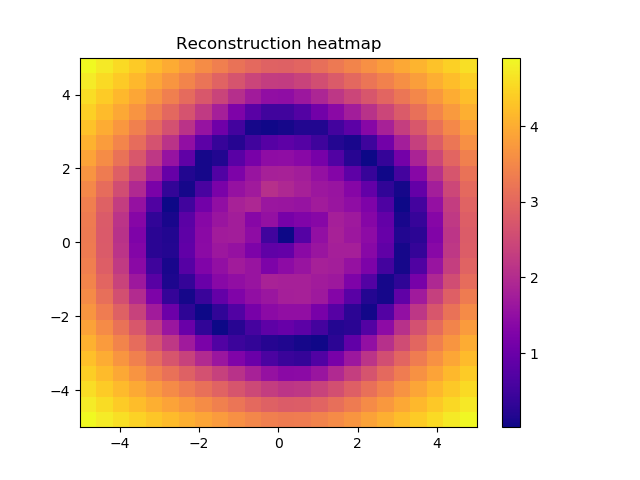
\includegraphics[width=.95\linewidth]{figures/circle-quantifier-reconstruction}
  \caption{Circle - Norm reconstruction error}
\end{subfigure}
\begin{subfigure}{.5\textwidth}
  \centering
  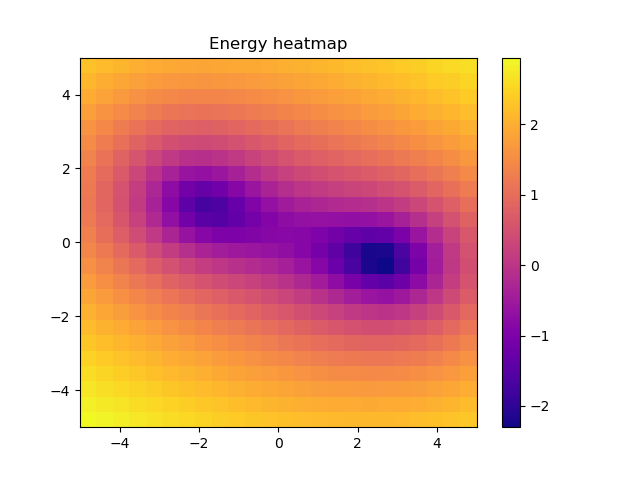
\includegraphics[width=.95\linewidth]{figures/wave-quantifier-energy}
  \caption{Wave - Potential energy}
\end{subfigure}%
\begin{subfigure}{.5\textwidth}
  \centering
  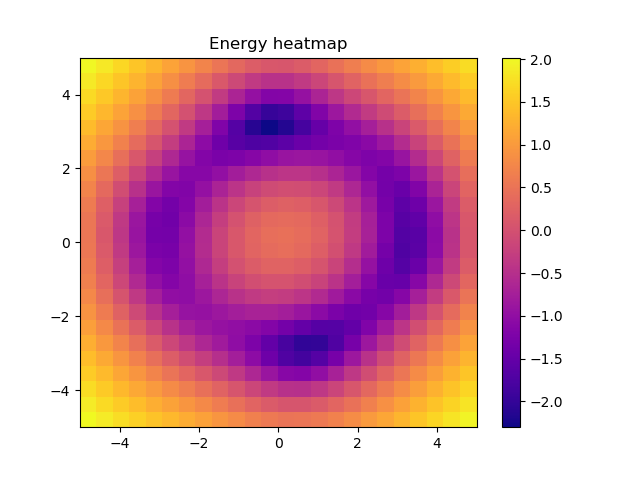
\includegraphics[width=.95\linewidth]{figures/circle-quantifier-energy}
  \caption{Circle - Potential energy}
\end{subfigure}
\caption[Heatmap of estimators on wave and circle manifold]{Estimators evaluated on wave (left) and circle (right) manifolds.}
\label{fig:exp1-heatmaps}
\end{figure}


%----------------------------------------------------------------------------------------
%	SECTION 
%----------------------------------------------------------------------------------------

\section{Limitations}

Many interesting data structures are difficult to reproduce with shallow denoising autoencoders. For example, sequential data (e.g. sound) is better modelled with LSTM-DAE\footnote{Long-Short Term Memory denoising autoencoder \citep{lstm-dae}}. Likewise, CNN-DAE\footnote{Convolutional Neural Network denoising autoencoder \citep{cnn-dae}} are more appropriate to model spatial structures, such as images. However, the integrability criterion for these models is not satisfied anymore, and thus the negative log-likelihood cannot be estimated. Alternative methods to efficiently learn energy functions for spatial or sequential data are presented in \citep{anomaly-detection-energy, energy-estimation}